\documentclass{beamer} % [aspectratio=169]
\usetheme{ucl}
\setbeamercolor{banner}{bg=darkred}
\setbeamersize{description width=2em}
\setbeamertemplate{navigation symbols}{\vspace{-2ex}} 
\usepackage{soul}

%\usepackage{fontspec}
\usepackage[utf8]{inputenc}
% \usepackage[english, greek]{babel}


\usepackage[T1]{fontenc} % Turn £ into $
\usepackage{minted}
\usemintedstyle{emacs}

\usepackage{fancyvrb}
\usepackage{xcolor}
\usepackage{url}

\usepackage{natbib}
\usepackage{bibentry}
\usepackage{url}


\usepackage{tikz}
\usetikzlibrary{positioning}
\usetikzlibrary{calc,shapes.multipart,chains,arrows}
\usetikzlibrary{shapes,snakes}

\tikzset{
  treenode/.style = {align=center, inner sep=0pt, text centered,
    font=\sffamily},
  arn_n/.style = {treenode, circle, draw=black,
     text width=1.5em},% arbre rouge noir, noeud noir
  arn_r/.style = {treenode, circle, red, draw=red, 
    text width=1.5em, very thick},% arbre rouge noir, noeud rouge
  arn_d/.style = {treenode, star, star points=10, red, draw=red, 
    text width=1.5em, very thick},% arbre rouge noir, noeud rouge
  arn_x/.style = {treenode, rectangle, draw=black}% arbre rouge noir, nil
}

\newcommand\emc[1]{\textcolor{midred}{\textbf{#1}}}

\AtBeginSection[]{
  \begin{frame}
  \vfill
  \centering
  \begin{beamercolorbox}[sep=8pt,center,shadow=true,rounded=true]{title}
    \usebeamerfont{title}\insertsectionhead\par%
  \end{beamercolorbox}
  \vfill
  \end{frame}
}

\author{Mark Handley, University College London\\
\small  based on slides from Prof.\ George Danezis}
\title{Develpment Practices}
\subtitle{ENGF0002: Design and Professional Skills }
% \institute{}
\date{Term 1, 2018}


\begin{document}
\nobibliography*


\frame{
\titlepage
}

\begin{frame}
\frametitle{Outline}

This topic is all about \emc{scaling up} the development process, while maintaining \emc{feasibility and quality}.

\begin{itemize}
  \item Traditional software \emc{development methods \& disasters}.
  \item The \emc{Agile} software development framework.
  \item \emc{Tools} to support development teams.
\end{itemize}

\end{frame}

\section{Traditional software development.}

\begin{frame}
\frametitle{Software development methods \& project management.}

Different than traditional engineering management:
\begin{itemize}
  \item Recent discipline, immature processes and tools \\ (\emc{incidental complexity}).
  \item \emc{Intrinsic complexity} increased through \emc{no physical constraints}.
  \item Tight integration between requirements, specification, implementation, operation -- no \emc{manufacturing} stage.
  \item Complexity increased through \emc{flexibility} -- ever changing \& evolving requirements.
  \item Difficult to \emc{estimate} time to completion \& defect rate.
  \item Orders of magnitude differences in \emc{programmer productivity}.
\end{itemize}

\end{frame}

\begin{frame}
\frametitle{Anti-pattern: The Waterfall model.}

Adapted from other engineering (construction). The \emc{Waterfall model} structures a project as a sequence of:
\begin{itemize}
\item \emc{Requirements gathering}
\item \emc{System Design \& Specification}. \\ Also known as `Big Design Up Front'.
\item \emc{Implementation}
\item \emc{Testing \& Validation}
\item \emc{Deployment \& Maintenance}
\end{itemize}

\begin{block}{}
\small Winston Royce (Director at Lockheed Software Technology Center) in 1970 presents the model as a `bad idea'. It is later (1985) formalized -- in terms of auditing steps -- as a methodology in US Dept.\ of Defense `Defense Systems Software Development' (DOD-STD-2167A). Subsequent MIL-STD-498 in 1994 states a preference for `Iterative and incremental development'.
\end{block}

\end{frame}

\begin{frame}
\frametitle{Problems with the Waterfall model.}

All activities included in the model need to take place at some point. However, a linear end sequential application is not appropriate, because:
\begin{itemize}
  \item \emc{Users do not know} or cannot formulate requirements, until they see working software (prototypes, early versions, \ldots)
  \item \emc{Designers may not foresee} all issues related to the implementation, or be able to chose between design options, without prototyping and testing.
  \item In case \emc{different people} are employed in different phases, \emc{communication breakdown} may occur; and only a \emc{fraction of the team is engaged} at any point.
\end{itemize}

Poorly adapted to \emc{`brown-field' development}, where existing software needs to be extended, rather than `green-field' new projects.

\end{frame}

\begin{frame}
\frametitle{The tar pit (Brooks 1975)}

\begin{center}
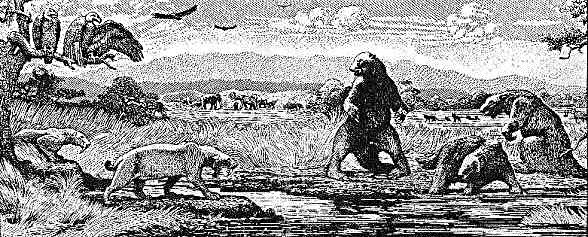
\includegraphics[scale=0.5]{assets/tar-pit}
\end{center}

{\small The Mythical Man-Month. Essays on Software Engineering by Frederick Brooks Jr. Anniversary Edition  Paperback, 322 pages Published by Addison-Wesley Pub Co in July 1995. (First edition 1975.)}

\end{frame}

\begin{frame}
\frametitle{Lessons from `The Mythical Man-Month' (1)}

Brooks was an architect on the IBM OS/360 -- delivered epically late in the 1970s.
\begin{itemize}
  \item  \emc{Brooks's law}: `\emph{Adding manpower to a late software project makes it later}'. The communication channels increase as $\mathcal{O}(n^2)$ in the number $n$ of developers.
  \item \emc{No silver Bullet}: No single development method, language or tool can reduce software dev. by an order of magnitude, since they may only reduce incidental not intrinsic complexity.
  \item \emc{The Second-System effect}: Be aware of the second version of a system, since the architects will try to include all options they did not include in the first.
\end{itemize}

\end{frame}

\begin{frame}
\frametitle{Lessons from `The Mythical Man-Month' (2)}

\begin{itemize}
  \item \emc{The Pilot system}: when designing a new system, plan for an initial pilot (prototype) which will help you learn. Throw it away, and deliver the second one.
  \item \emc{Project estimation}: programming products take much longer to build, than internal tools; a lot of time is taken by communications, `stand-ups' and `all-hands'.
  \item \emc{The surgical team}: Build small teams around and supporting experienced programmers.
  \item \emc{Code freeze}: freeze features at some point, and only increase the quality of code, until next release.
\end{itemize}

\end{frame}

\begin{frame}
\frametitle{Spiral model to manage risk.}

\begin{center}
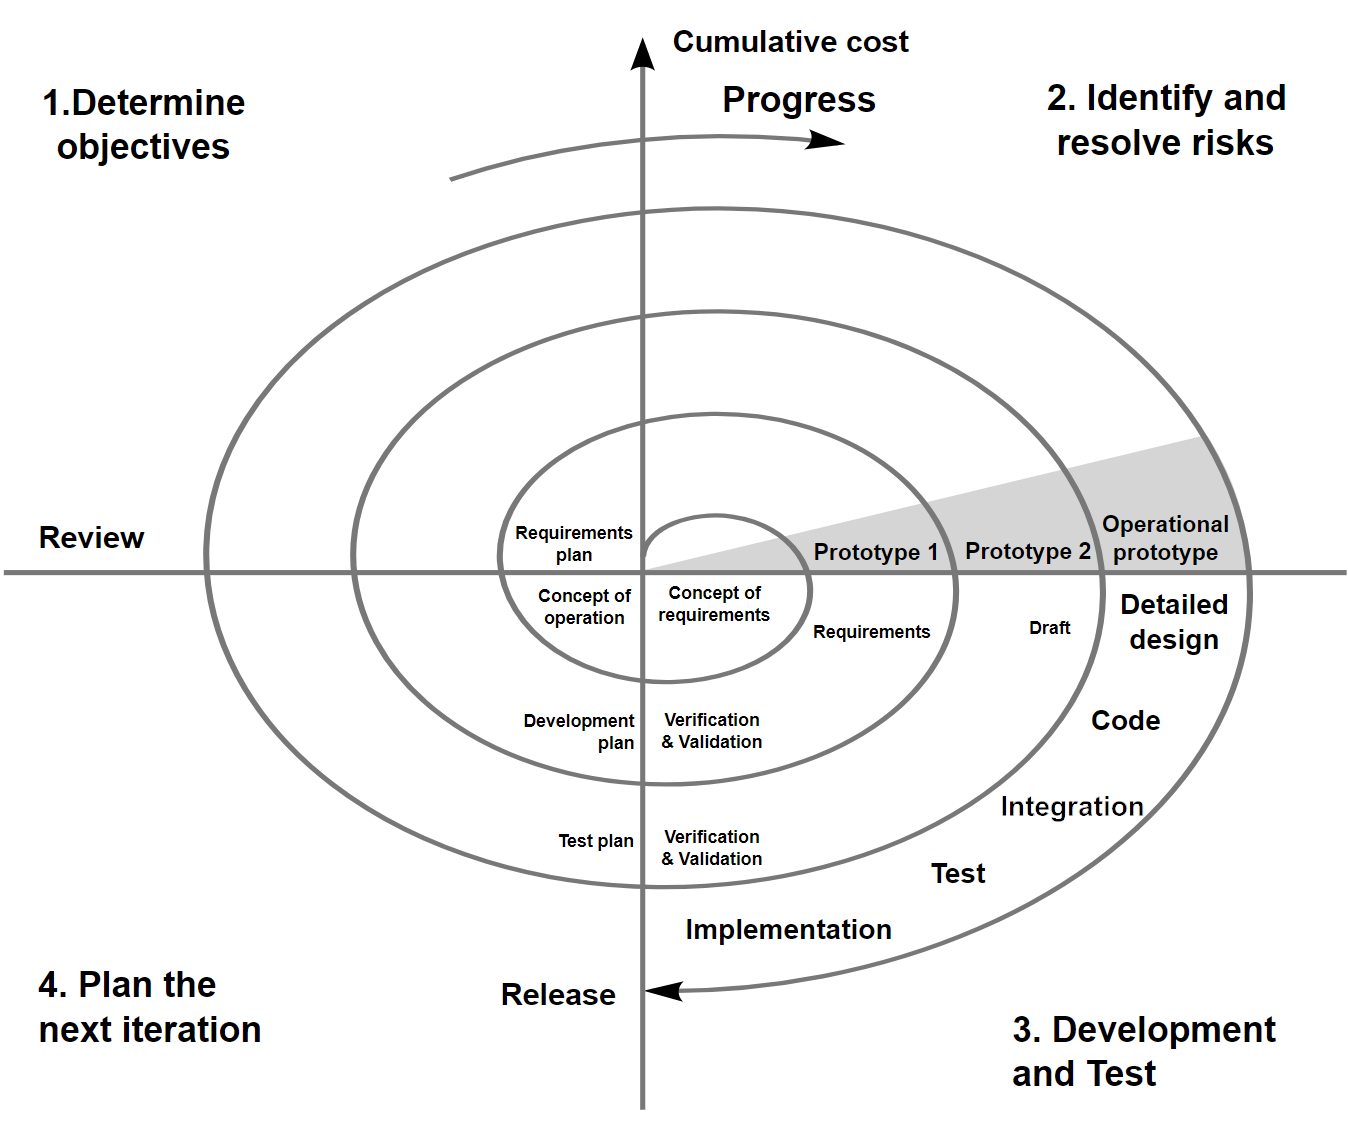
\includegraphics[scale=0.27]{assets/spiral}
\end{center}

{\small Boehm ``A Spiral Model of Software Development and Enhancement'', ACM SIGSOFT Software Engineering Notes, ACM, 11(4):14-24, August 1986}

\end{frame}

\section{Agile development and practices.}

\begin{frame}
\frametitle{The Manifesto for Agile Software Development (2001).}

Radical: Re-focus on \emc{software as working code}: `The need for an \emc{alternative to documentation driven, heavyweight} software development processes.'

\vspace{5mm}
Why the crisis? Traditional software \emc{project failures} in 1995:
\begin{itemize}
  \item 16.2\% -- Project Success: on time, budget, features.
  \item 52.7\% -- Project Challenged: overrun time, budget, fewer features.
  \item 31.1\% -- Project Impaired: canceled at some point.
\end{itemize}
 (Standish Group, CHAOS Report, 1995)

\end{frame}

\begin{frame}
\frametitle{The Manifesto (1--6).}


\begin{itemize}
\item Our highest priority is to satisfy the customer
through \emc{early and continuous delivery
of valuable software}.

\item Welcome \emc{changing requirements, even late} in 
development. 

\item Deliver \emc{working software} frequently, from \emc{a 
couple of weeks to a couple of months}, with a 
preference to the shorter timescale.

\item \emc{Business people} and \emc{developers must work 
together} daily throughout the project.

\item Build projects around \emc{motivated individuals}. 
Give them the support they need, 
and \emc{trust them} to get the job done.

\item The most efficient and effective method of 
conveying information to and within a development 
team is \emc{face-to-face conversation}.

\end{itemize}

\end{frame}

\begin{frame}
\frametitle{The Manifesto (7--12).}

\begin{itemize}


\item \emc{Working software is the primary measure of progress}.

\item Agile processes promote \emc{sustainable development}. 
The sponsors, developers, and users should be able 
to maintain a \emc{constant pace indefinitely}.

\item Continuous attention to \emc{technical excellence 
and good design enhances agility}.

\item Simplicity--the art of \emc{maximizing the amount 
of work not done}--is essential.

\item The best architectures, requirements, and designs 
emerge from \emc{self-organizing teams}.

\item At regular intervals, the team \emc{reflects on how 
to become more effective}, then tunes and adjusts 
its behavior accordingly.

\end{itemize}

\end{frame}


\begin{frame}

\frametitle{Composition of an Agile team}

\begin{itemize}
\item \emc{The product manager / owner} -- Maintain and promote the product vision. Part management, part people coordination, part marketing.

\item \emc{On-site customers} -- team members representing customers, continuously capturing and discussing requirements, and discussing with programmers. \\ Can be business people. Incl. 2 per 3 programmers!

\item \emc{Programmers} -- Bulk of the team, no distinction between `architects', `developers', `testers'. Incl.\ one senior, hands-on, person and overall teams of 4--9 programmers. Although some members may have a focus.

\item \emc{Domain experts, Interaction Designers, Security, Design, and Business Analysts} -- experts in their respective domains, are on-call to help on-demand. Work with both users and team.

\end{itemize}

\end{frame}


\begin{frame}
\frametitle{Ratio of on-site customers to programmers}

Do you think the ratio is too high or too low?

\vspace{5mm}
What processes do user representatives speed up?

\end{frame}



\begin{frame}
\frametitle{The rhythm of an Agile project -- Sprints}

``You can eliminate requirements, design, and testing phases as well as the formal documents that go with them.''

\begin{center}
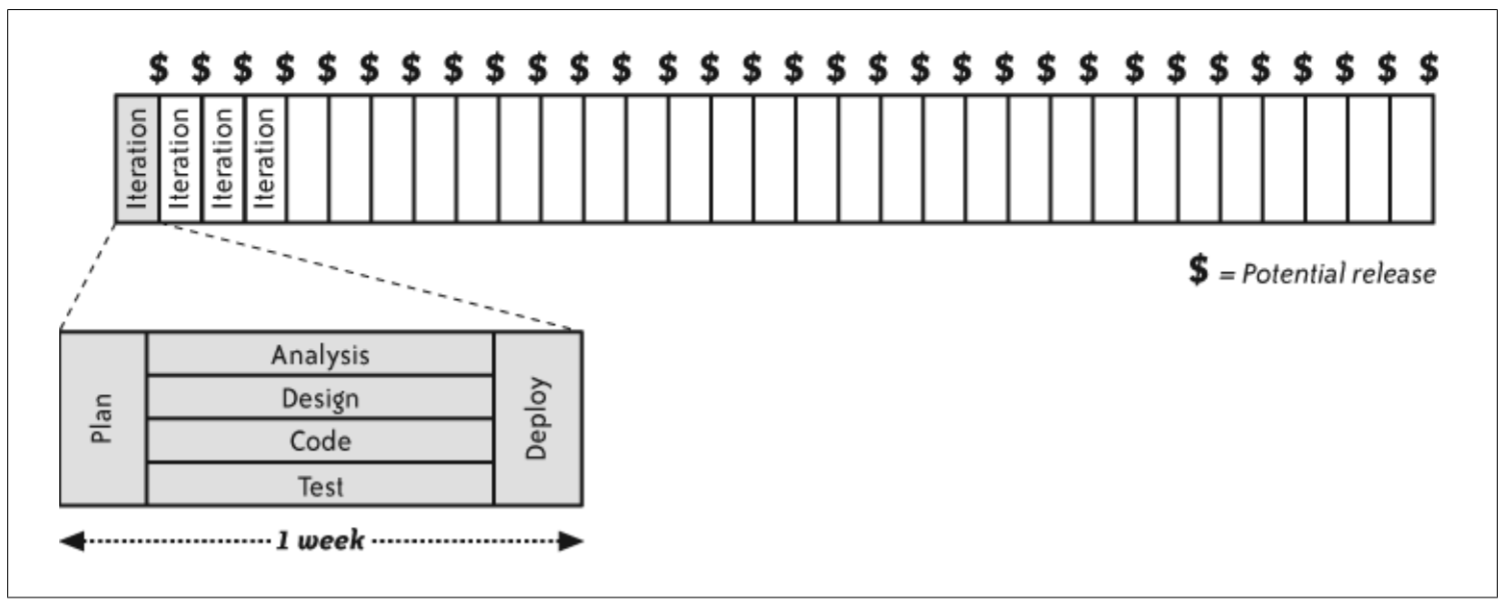
\includegraphics[scale=0.35]{assets/agile} \\
Agile (XP) Lifecycle. Sprints are typically 1-2 weeks.
\end{center}

{\small The Art of Agile Development by James Shore. Wiley 2007.}

\end{frame}


\begin{frame}

\frametitle{User Stories}

Stories represent \emc{self-contained, individual elements} of the project: 
\begin{itemize}
\item Individual features.
\item Typically represent one or two days of work.
\item Customer-centric, in terms of business results.
\item No implementation details, or full requirements / specifications.
\end{itemize}

\vspace{5mm}
Good user stories have the form: \\ \emc{As a {\em <type of user>} I want {\em <some goal>} so that {\em <some reason>}}.

\end{frame}

\begin{frame}
  \frametitle{User Stories}
  E.g. a high level user story example for a laptop backup product:

  \begin{itemize}
  \item {\em As a user, I can backup my entire hard drive.}
    \end{itemize}

  So called ``epic'' user stories are usually split into smaller user stories before they are worked on:
  \begin{itemize}
   \item {\em As a power user, I can specify files or folders to backup based on file size, date created and date modified.}
   \item {\em As a user, I can indicate folders not to backup so that my backup drive isn't filled up with things I don't need saved}
  \end{itemize}
\end{frame}


\begin{frame}

\frametitle{Backlogs: Product, Release \& Sprint}

All stories are stored in the \emc{product backlog}:
\begin{itemize}
  \item When a new release is planned / discussed with customers some stories are moved to the \emc{release backlog}. They are augmented by \emc{acceptance criteria}.
  \item At the start of every sprint, some stories are moved into the \emc{sprint backlog}, along with noted on \emc{how to design \& implement} them.
  \end{itemize}

Programmers are asked to `cost stories' in `days', as stories progress through backlogs:
\begin{itemize}
  \item Programmers are bad at estimating, but their estimates are \emc{off by a fixed multiplicative constant}.
  \item \emc{Velocity}: the number of story `days' the project executes (Done Done!) in a day. Base \emc{project estimation} on velocity.
\end{itemize} 

\end{frame}


\begin{frame}

\frametitle{Backlogs \& stories: just a bunch of post-its or cards}

\begin{center}
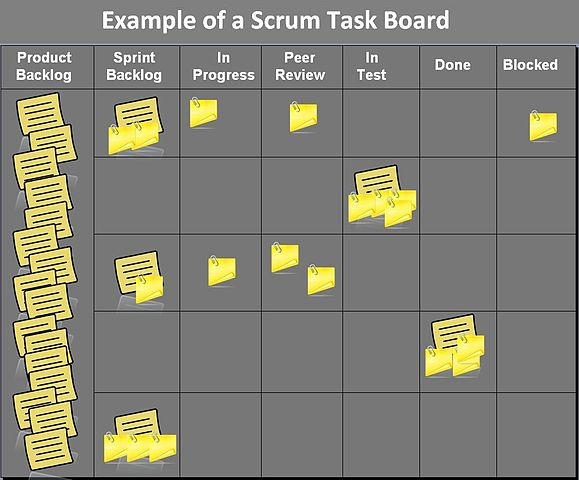
\includegraphics[scale=0.50]{assets/backlog} 
\end{center}


`Kanban' board. From \url{https://dzone.com/articles/product-backlogs-practice/}

\end{frame}


\begin{frame}

\frametitle{On-line tools for Agile project management.}

A number of tools can \emc{replace physical post-it notes}:
\begin{itemize}
  \item Trello (hip) -- \url{http://trello.com}.
  \item Github projects -- see `Projects' tab on your project page.
\end{itemize}

\vspace{5mm}
Related but different tool: \emc{Issue / Bug tracker.}
\begin{itemize}
  \item Allow users, internal and external developers to \emc{report issues}.
  \item Allows \emc{discussion} on the issue and the development of a \emc{minimal test case to reproduce the error}.
  \item Allows for \emc{triage}, and \emc{assignment} of issues to team members.
  \item Can be `abused' to report feature requests, and simulate a story board.
  \end{itemize}

\end{frame}

\begin{frame}

\frametitle{Agile practices: Pair programming}

Two programmers work together on a \emc{single workstation}. 
\begin{itemize}
\item One \emc{driver / codes} the other \emc{navigator / reviews \& thinks}.
\item They \emc{switch roles} frequently.
\end{itemize}

Why pair?
\begin{itemize}
  \item Navigator has opportunity to think about \emc{strategic design} choices. Driver can focus on  \emc{code tactics}. Higher quality code.
  \item Reinforces, and shares \emc{good programming habits}. Continuous testing and refinement result from \emc{peer pressure}.
  \item Resilient to \emc{interruptions}. When interrupted one person can handle interrupt, while other codes.
  \item Its \emc{more fun} to not work alone. Can take \emc{physical breaks}.
\end{itemize}
Focus on sustaining, rather than peaks of high production.

\end{frame}


\begin{frame}
\frametitle{Pair programming or code reviews?}

What do the practices have in common?

\vspace{5mm}
What are their advantages and disadvantages?

\end{frame}



\begin{frame}

\frametitle{Agile practices: Documentation \& Agile Modeling.}

Keep the non-code project documentation to a minimum.
\begin{itemize}
\item \emc{Document continuously}: \emc{Minimal} stories, design notes and meeting notes.
\item \emc{Document late}: Do now write anything that will not be read or acted upon. Minimize speculation.
\item \emc{Single Source Information}: All project \emc{documentation} has to be \emc{kept under version control}.
\item \emc{Prefer Executable specifications}: Write as \emc{customer tests} that can execute against the code. (TDD at the requirements level.)
\end{itemize}

\vspace{5mm}
All code and docs is kept in version control.
\end{frame}

\begin{frame}

\frametitle{Agile practices: Distributed Version Control.}

Use Distributed Version Control for \emc{fearless refactoring} and \emc{collaborative coding}:
\begin{itemize}
  \item Tool of choice: \texttt{git} and \texttt{github}.
  \item Code lives in \emc{repositories}, \emc{remote} and \emc{local}.
  \item A repository can have multiple \emc{branches}. 
  \item You may \emc{branch} and \emc{merge}, or \emc{commit} code to a branch.
\end{itemize}

\vspace{5mm}
\emc{Learn git!} \url{https://git-scm.com/documentation/external-links} 

\vspace{5mm}
Gitflow illustrations by Vincent Driessen \url{http://nvie.com}.


\end{frame}


\begin{frame}
\frametitle{Agile practices: Gitflow \& version control.}

A \emc{branch} in a git repository contains a `variant' of your repository. You can \emc{merge} a branch into another, after a number of \emc{commits}.

\vspace{5mm}
Gitflow basic organization for a repository:
\begin{itemize}
  \item The \emc{master} branch only contains tagged releases.
  \item A \emc{develop} branch is used to continuously update the software.
  \item New features are developed in separate \emc{feature} branches.
  \item A \emc{release branch} captures the features for a new release, and from there on only accepts \emc{bug fixes}.
  \item Eventually a release branch is merged into master to make a new release.
  \item \emc{Hotfixes} are applied to master and merged into develop. 
  \end{itemize}

Good programmers use it even when they work on their own!
\end{frame}


\begin{frame}
\begin{center}
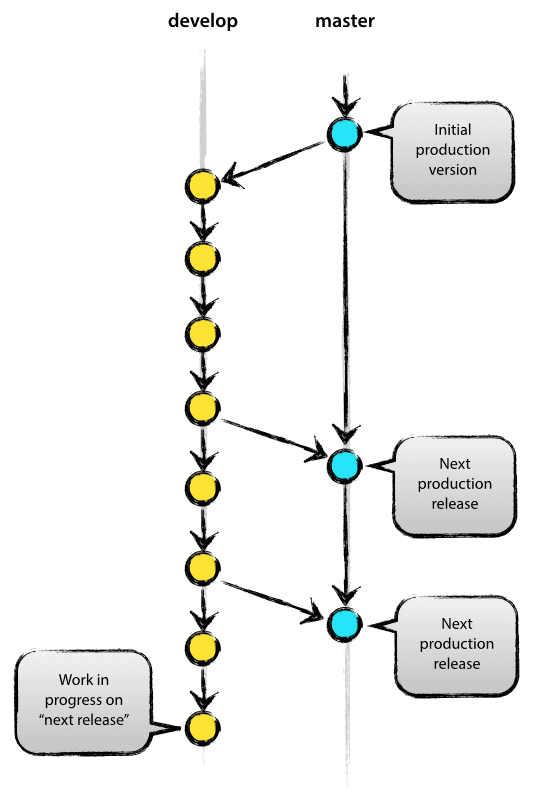
\includegraphics[height=80mm]{assets/main-branches}
\end{center}
\end{frame}

\begin{frame}
\begin{center}
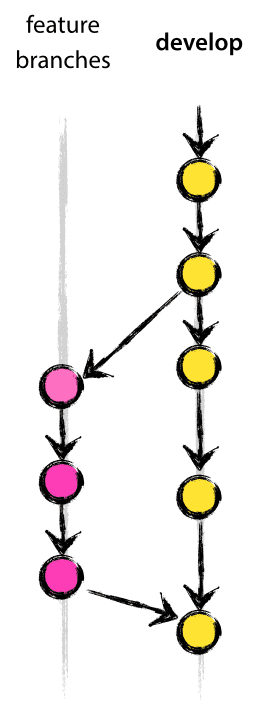
\includegraphics[height=80mm]{assets/feature-branches} 
\end{center}
\end{frame}

\begin{frame}
\begin{center}
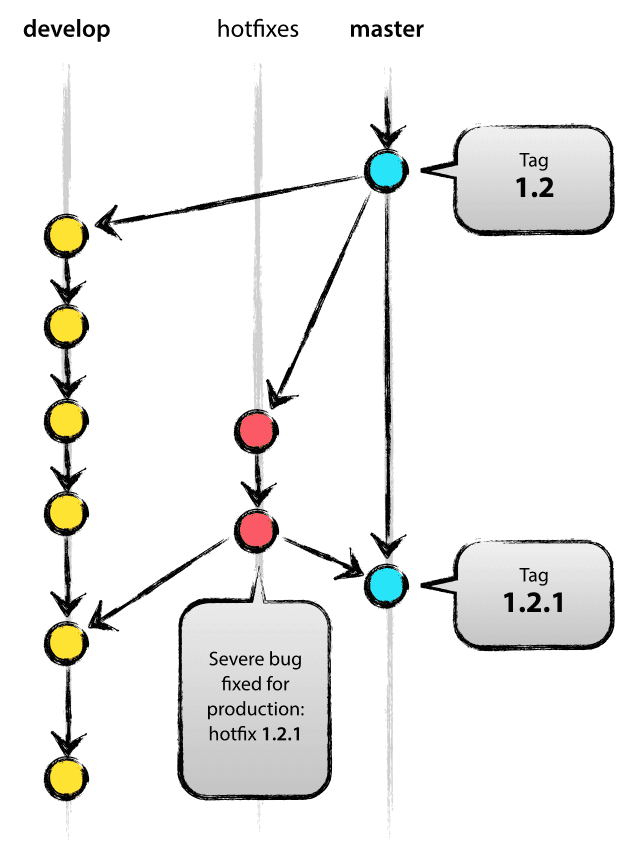
\includegraphics[height=80mm]{assets/hotfix-branches} 
\end{center}
\end{frame}

\begin{frame}
\begin{center}
\includegraphics<1>[scale=0.33]{assets/flow00} 
\includegraphics<2>[scale=0.33]{assets/flow0} 
\includegraphics<3>[scale=0.33]{assets/flow1} 
\includegraphics<4>[scale=0.33]{assets/flow2} 
\includegraphics<5>[scale=0.33]{assets/flow3} 
\end{center}

\end{frame}

\begin{frame}

\frametitle{Why different feature branches?}

Why develop different user stories on different feature branches?

\vspace{5mm}
What is the cost of diverging too much from the develop branch?

\vspace{5mm}
How do you ensure you do not diverge too much from the develop branch?

\end{frame}


\begin{frame}
\frametitle{Agile practices:`Done Done'.}

Each feature branch represents a user story, and it is merged into develop when it is `\emc{done done}.':
\begin{itemize}
  \item Fully Designed, Coded, Integrated (from UI to Database), Tested (unit, integration, and customer tests finished).
  \item Builds, Installs (incl. auto install \& devops), Migrates past state.
  \item Fixed all bugs, Reviewed by customers and accepted as finished.
\end{itemize}

\begin{block}{From working software to working software}
Executing each user story until it is `done done' takes working software and produces working software, end-to-end. This way users can see progress and provide early feedback.
\end{block}

\end{frame}

\begin{frame}
\frametitle{Agile practices:Continuous Integration.}

\begin{block}{The `build' engineer}
Merging branches that are a lot of different commits apart, is time consuming. At traditional software firms this is the job of the `build' engineer. `Integration' and testing of different branches can take months.
\end{block}

\vspace{3mm}
\emc{Continuous Integration}: be technically ready to release, even if you are not functionally ready.
\begin{itemize}
  \item Create automated pipeline for testing integration, packaging, installers, deployment in servers, and data migration.
  \item Run those tests on every commit to develop branch.
  \end{itemize}


\end{frame}

\begin{frame}

\frametitle{Why testing continuously?}

Integration, Install, Deployment, Migration: even when the features are not entirely finished or there?

\end{frame}

\begin{frame}

\frametitle{Other Agile practices}

Other tricks of the trade:
\begin{itemize}
  \item Test driven development.
  \item Agile testing \\ (specification by example.)
  \item Refactoring.
  \item Cross-functional teams.
  \item Information Radiators.
  \item Planning poker.
  \item Scrum events \\ (planning, daily Stand-up meetings).
  \item Timeboxing.
\end{itemize}

\end{frame}

\begin{frame}
\frametitle{Conclusion: `No silver bullet'.}

\begin{center}
\includegraphics<1>[scale=0.90]{assets/agilewaterfall} \\
{\tiny from \url{https://www.infoq.com/articles/standish-chaos-2015}}
\end{center}


\end{frame}

\bibliographystyle{alpha}
\nobibliography{references}

\end{document}
